\documentclass[12pt]{article}

\usepackage[utf8]{inputenc}
\usepackage[english]{babel}
\usepackage{fancyhdr}
\usepackage{graphicx}
\graphicspath{ {./images/} }
\usepackage{titling}
\usepackage{wrapfig}
\usepackage{float}
\usepackage[table,xcdraw]{xcolor}
\usepackage{blindtext}
\usepackage{setspace}
\usepackage{listings}
\usepackage{tocloft}
\usepackage{placeins}
\usepackage[titletoc]{appendix}
\usepackage{etoolbox}
\usepackage{setspace}
\usepackage{makecell, caption}
\renewcommand\theadfont{\normalsize\bfseries\boldmath}
\usepackage{siunitx}
\sisetup{detect-weight, range-phrase=/, range-units = single}
\usepackage{lipsum}
\usepackage{amsmath,amssymb}
\usepackage{caption}
\usepackage{subcaption}
\usepackage{commath}
\usepackage{float}

\usepackage[T1]{fontenc}                
\usepackage{booktabs}

\doublespacing
\usepackage[
    backend=biber,
    style=mla-new,
    citestyle=authoryear
    ]{biblatex}
\addbibresource{sources.bib}

\usepackage{geometry}
 \geometry{
 a4paper,
 left=15mm,
 right=15mm,
 bottom=20mm,
 top=20mm,
 }

\pagestyle{fancy}
\fancyhf{}
\chead{
        \textsc{The Damping Ratio of an Airplane Wing Relative to its Length}
    }
\rfoot{Page \thepage}

\begin{document}

\section{Exploration}

\subsection{Introduction}

As an aspiring aerospace engineer, understanding how different factors of a plane affect the flight is imperative for designing aircrafts. Plane wings are designed to naturally bend when unbalanced forces are applied, such as an net upwards lift force generated from air currents or changes in air density. This causes components of the airplane, like the wings, to exhibit simple harmonic motion for a period of time as they return to equilibrium after bending. The stiffness of the materials used in aircrafts are specifically chosen to minimise vibrations that occur as a result of these unbalanced forces during the flight by creating a damped oscillating effect (\citeauthor{anderson_bowden_2022}). However, I was interested in investigating rather how the length of a plane wing itself affected this same property since the spring coefficient of a material is also related to the distance from equilibrium of the applied force, leading me to the research question: \textbf{How does the length of an airplane wing affect the damping ratio of the oscillating structure?}


\subsection{Theoretical Background}

\subsubsection{Stability}
The nature of a plane wing to initially tend towards its equilibrium position after being disturbed by an unbalanced force is referred to as its static stability (\citeauthor{anderson_bowden_2022}). There are three types of static stability: statically stable, statically neutral, and statically unstable. Statically stable objects, when disturbed by a force, will initially tend towards their equilibrium position, whereas statically neutral objects will remain in equilibrium even after being disturbed by a force. On the other hand, statically unstable objects will tend away from their equilibrium after having a force applied. The concept of static stability can be simplified with a marble in a bowl analogy depicted below in Figure \ref{fig:static.stability}, where a statically stable marble will initially tend towards the centre of the bowl because of the restoring gravitational force, while the statically neutral marble will not have any restoring force, and the statically unstable marble will tend away from the centre of the bowl because of the gravitational force pulling it away. In the case of the plane wing, this restoring force is the spring energy from the stiffness of the wing material. Designing a plane wing with static stability is imperative for its response to unbalanced forces. 

\begin{figure}[h]
     \centering
     \begin{subfigure}[b]{0.3\textwidth}
         \centering
         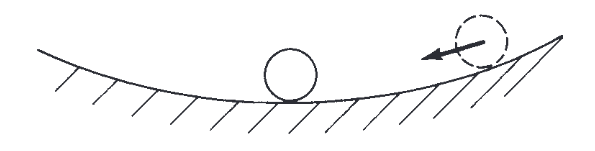
\includegraphics[width=\textwidth]{images/positive static.png}
         \caption{Statically stable}
         \label{fig:s.stable}
     \end{subfigure}
     \hfill
     \begin{subfigure}[b]{0.3\textwidth}
         \centering
         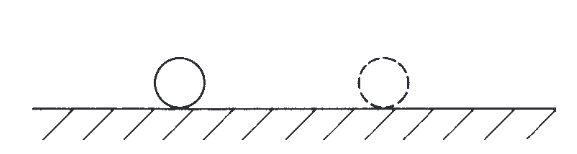
\includegraphics[width=\textwidth]{images/statically neutral.png}
         \caption{Statically neutral}
         \label{fig:s.neutral}
     \end{subfigure}
     \hfill
     \begin{subfigure}[b]{0.3\textwidth}
         \centering
         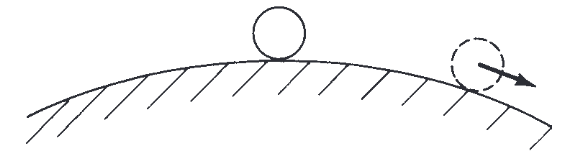
\includegraphics[width=\textwidth]{images/statically unstable.png}
         \caption{Statically unstable}
         \label{fig:s.unstable}
     \end{subfigure}
     \hfill
        \caption{Different types of stability illustrated by marbles (\citeauthor{anderson_bowden_2022})}
        \label{fig:static.stability}
\end{figure}

However, what happens after a plane wing initially responds to this unbalance is the dynamic stability. A plane wing responding with damped oscillations to an external force is said to be dynamically stable (\citeauthor{anderson_bowden_2022}). There also exists the case where an object may be dynamically unstable, where the plane wing oscillates with increasing amplitude, regardless of its static stability as this is only relevant for the initial tendency. Dynamic neutrality, where an object remains in simple harmonic motion is only theoretically possible due to energy losses in the system of the plane wing. These can be graphed as show below in Figure \ref{fig:dynamic.stability}, with variations in the sinusoidal functions. For an airplane wing, a dynamically stable system, with a high damping constant is desirable as it allows the plane wing to return to equilibrium after being disturbed.

\begin{figure}[h]
     \centering
     \begin{subfigure}[b]{0.3\textwidth}
         \centering
         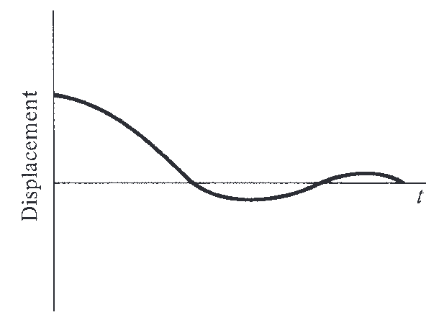
\includegraphics[width=\textwidth]{images/d stable.png}
         \caption{Dynamically stable}
         \label{fig:d.stable}
     \end{subfigure}
     \hfill
     \begin{subfigure}[b]{0.3\textwidth}
         \centering
         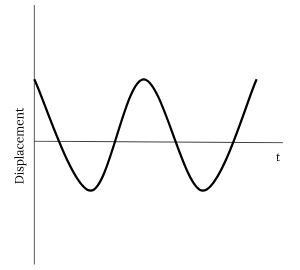
\includegraphics[width=\textwidth]{images/d neutral.png}
         \caption{Dynamically neutral}
         \label{fig:d.neutral}
     \end{subfigure}
     \hfill
     \begin{subfigure}[b]{0.3\textwidth}
         \centering
         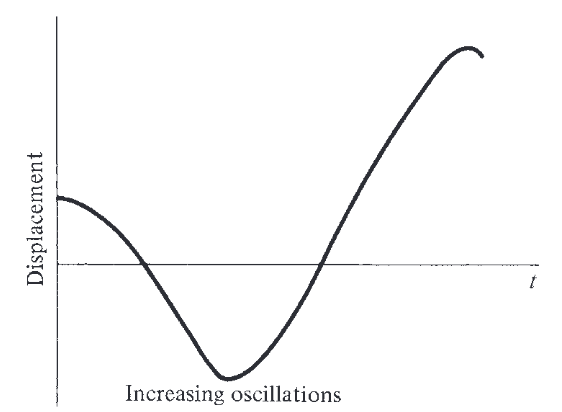
\includegraphics[width=\textwidth]{images/d unstable.png}
         \caption{Dynamically unstable}
         \label{fig:d.unstable}
     \end{subfigure}
     \hfill
        \caption{Graphical representations of dynamic stability (\citeauthor{anderson_bowden_2022})}
        \label{fig:dynamic.stability}
\end{figure}


\subsubsection{Simple Harmonic Motion}
These sinusoidal oscillations are an example of simple harmonic motion - the periodic movement of an object about an equilibrium without the presence of a net force (\citeauthor{britannica_2023}). Depending on the material, these oscillations can either be damped or excited, as demonstrated by dynamically stable and unstable systems in Figure \ref{fig:dynamic.stability} respectively. As the plane wing is displaced by an unbalanced force, its statically stable nature will allow it to have an initially tendency to return to equilibrium, and as a dynamically stable system, the restoring forces from the spring constant of the material will dampen its oscillations. As the spring constant is a quantity related to distance (measured in $\frac{N}{m}$), changes in the length of the plane wing will have a direct relationship with the amount of potential energy stored in the system given a displacement from the equilibrium. Since this is a statically and dynamically stable system, the damping ratio, $\zeta$, as a dimensionless measure of how the oscillatory system decays, will be investigated as a measure of how the length of a plane wing affects the oscillatory motion. 

\subsubsection{Mathematical Methods}
As we are dealing with an underdamped system, that is, one that returns to equilibrium after oscillating through the equilibrium with increasingly less energy each time, the oscillations can be modelled by a logarithmic decrement function in Figure \ref{fig:log.dec}.

\begin{figure}[h]
    \centering
    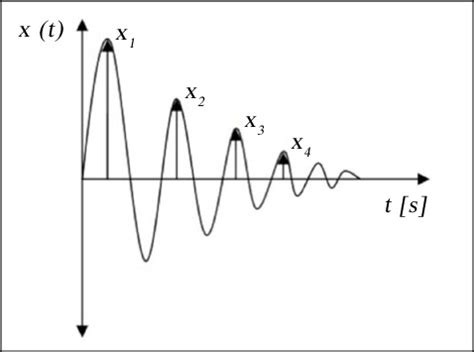
\includegraphics[scale=0.5]{images/log dec.jpg}
    \caption{Logarithmic Decrement Function (\citeauthor{jovanović_simonovic_lukić_zorić_stup_ilić_2014})}
    \label{fig:log.dec}
\end{figure}

Using this function we can consider how the amplitude of each wave peak changes with each oscillation, which can be modelled by an exponential function. Hence, we can take the natural logarithm of each peak amplitude and model their differences as a logarithmic decrement, $\delta$, where $A_1$ is the initial amplitude and $A_2$ is the amplitude of the subsequent oscillation (Equation \ref{log.dif}):

\begin{equation}\label{log.dif}
    \delta = \ln(A_1) - \ln(A_2) = \ln(\frac{A_1}{A_2})
\end{equation}

From the equation for the logarithmic decrement, $\delta$, from MIT Mathematics 18.03's supplemental coursework below:

\vspace{-5mm}

\begin{equation}
    \delta = \frac{2\pi\zeta}{\sqrt{1-\zeta^2}}
\end{equation}

We can solve for the damping ratio, $\zeta$, in terms of our logarithmic decrement, $\delta$, to demonstrate the relationship between the change in oscillation amplitude and damping ratio:

\begin{equation}\label{zeta in delta}
    \zeta = \frac{\delta}{\sqrt{4\pi^2+\delta^2}}
\end{equation}

We can now observe the relationship between natural angular frequency ($\omega_n$) and the spring constant ($k$) in an undamped system, where $T$ is period and $m$ is the mass in the system to find the proportionality between $k$ and $\omega_n$.

$$
\begin{array}{l|c}
    \omega_n = \frac{2\pi}{T} & \text{Angular frequency equation} \\ \\
    T = 2\pi \sqrt{\frac{m}{k}} & \text{Period equation} \\ \\
    \omega_n = \sqrt{\frac{k}{m}} & \text{Substituting } T \\ \\
 \end{array} 
$$

\begin{equation}\label{wnk}
    \boxed{\omega_n \propto \sqrt{k}}  \quad \text{Finding the proportionality}
\end{equation}

Using the equation for damped angular frequency, $
\omega_d$, from MIT Mathematics, we can see relationship between natural and damped angular frequencies, and how it is modified by $\zeta$ below:

\begin{equation}\label{wnwd}
    \omega_d = \omega_n\sqrt{1-\zeta^2}
\end{equation}

\subsection{Methodology}
As the effect of the length of a plane wing on the dampening ratio of the underdamped system is being investigated, firstly, the plane wing must be modelled. A 1 m wooden ruler is a highly simplified construction of a plane wing, however, since wood is often used in model airplanes because its structural flexibility and stiffness mimics that of actual aircrafts (\citeauthor{lacayo_2021}), a wooden ruler is an appropriate model for a plane wing while also being convenient. 

A preliminary experiment was conducted and it was determined that displacing the plane wing model to a constant vertical position did not produce consistent oscillations due to the difficulty in bending the wooden ruler at shorter lengths. Hence, placing a mass on the far end of the plane wing model allows us to maintain a constant restoring force since the gravitational force of the mass is displacing the plane wing model. It is important to note that the initial vertical displacement will change, however, this will be proportional to the change in spring constant as a result of the shortened length. 

A motion detector will be used to record the acceleration of the plane wing model, allowing us to produce an acceleration-time graph. We can graph the average of 7 trials for each measured length and qualitatively find the maxima of the first two oscillations. From these the logarithmic decrement, and subsequently damping ratio can be calculated for each length. Finally, length can be graphed against the damping ratio to find the relationship between these two variables. 


\section{Experimentation}
\subsection{Research Question and Hypothesis}

How does the damping ratio of an underdamped plane wing system change with the length of the plane wing (50.00 cm, 60.00 cm, 70.00 cm, 80.00 cm, 90.00 cm) as measured by the change in acceleration between two oscillatory maxima? 

As the length of the model airplane wing decreases, the damping ratio, $\zeta$, to maintain the underdamped system will increase. This is because the spring constant, $k$, of the model wing will increase since the applied force from the mass is constant (and $k$ is measured in $\frac{N}{m}$). Since natural angular frequency, $\omega_n$, is proportional to the square root of the spring constant (Equation \ref{wnk}), as $k$ increases, the $\omega_n$ will also increase. This will in turn result in the damped angular frequency, $\omega_d$, increasing because $\omega_n$ and $\omega_d$ are directly proportional as shown in Equation \ref{wnwd}. Hence, the damping ratio, $\zeta$, required to maintain the $\omega_d$ in the underdamped system will also increase. 

\subsection{Variables}

    \textbf{Independent variable:} The length of the model plane wing (90.00 cm, 80.00 cm, 70.00 cm, 60.00 cm, 50.00 cm), measured with a meter ruler ($\pm$0.05 cm).
    
    \noindent\textbf{Dependent variable:} The vertical acceleration in meters per second squared ($\pm 0.001 \frac{m}{s^2}$) of the model plane wing as measured by a Vernier Motion Detector. 
    
\subsection{Controlled variables}

\vspace{-2mm}

\begin{table}[H]
\centering
\caption{Controlled variables and their respective potential impact on the data collected and method to control to limit impact on data.}\label{controlled}
\begin{tabular}{|p{0.15\linewidth}|p{0.4\linewidth}|p{0.4\linewidth}|}
\hline
\rowcolor[HTML]{C0C0C0} 
    \multicolumn{1}{|c|}{Variable} 
    & \multicolumn{1}{|c|}{Potential Impact} 
    & \multicolumn{1}{|c|}{Method to Control} \\ 
\hline
    Magnitude of restoring force
    & If the restoring force changes, then the initial displacement from equilibrium of the plane wing model will change, as per Hooke's Law. This changes the vertical displacement measured, which will then change the logarithmic decrement, and hence, damping ratio. & A 200 g mass attached to a rubber band will be taped 5.00 cm ($\pm0.05$ cm) from the end of the plane wing model so that the same amount of gravitational force acts as the restoring force. The rubber band will be cut in one swift motion with scissors to ensure that the mass falling does not interfere with the oscillating plane wing. \\ 
\hline
    Plane wing model material stiffness 
    & The spring constant is a measurement of a material's stiffness, hence, if the material itself changes, it will have a different spring constant at the same lengths, changing the amount the plane wing is displaced by, and hence the logarithmic decrement and damping ratio. & A 1 m wooden ruler will be consistently used to model the plane wing in each trial to ensure that the stiffness of the material is the same, and hence, changes in the spring constant are attributed to the length of the plane wing, rather than changes in material. \\
\hline 
    Iterations per second of recorded data
    & If the number of iterations per second changes, the data's accuracy will change, where rapid changes displacement will not appear with less data points. & The motion detector will be set to record 100 data points per second at the beginning of each trial to ensure most consistent data. \\
\hline
    Calibration of the motion detector
    & If the motion detector is not calibrated, the initial displacement may be misread, hence impacting the calculated logarithmic decrement and damping ratio. & The motion detector will be repositioned above the plane wing model and calibrated to 0 at the beginning of each trial. \\
\hline
    Security of the plane wing model
    & If the model is not secured to the table, it may move with the oscillations causing energy losses external to the damping system, hence affecting the damping ratio. & The wooden ruler will be secured with tape and held down firmly with at least one hand during all trials. \\
\hline
\end{tabular}
\end{table}

\vspace{-4mm}

\subsection{Apparatus}

\vspace{-7mm}

\begin{figure}[H]
    \centering
    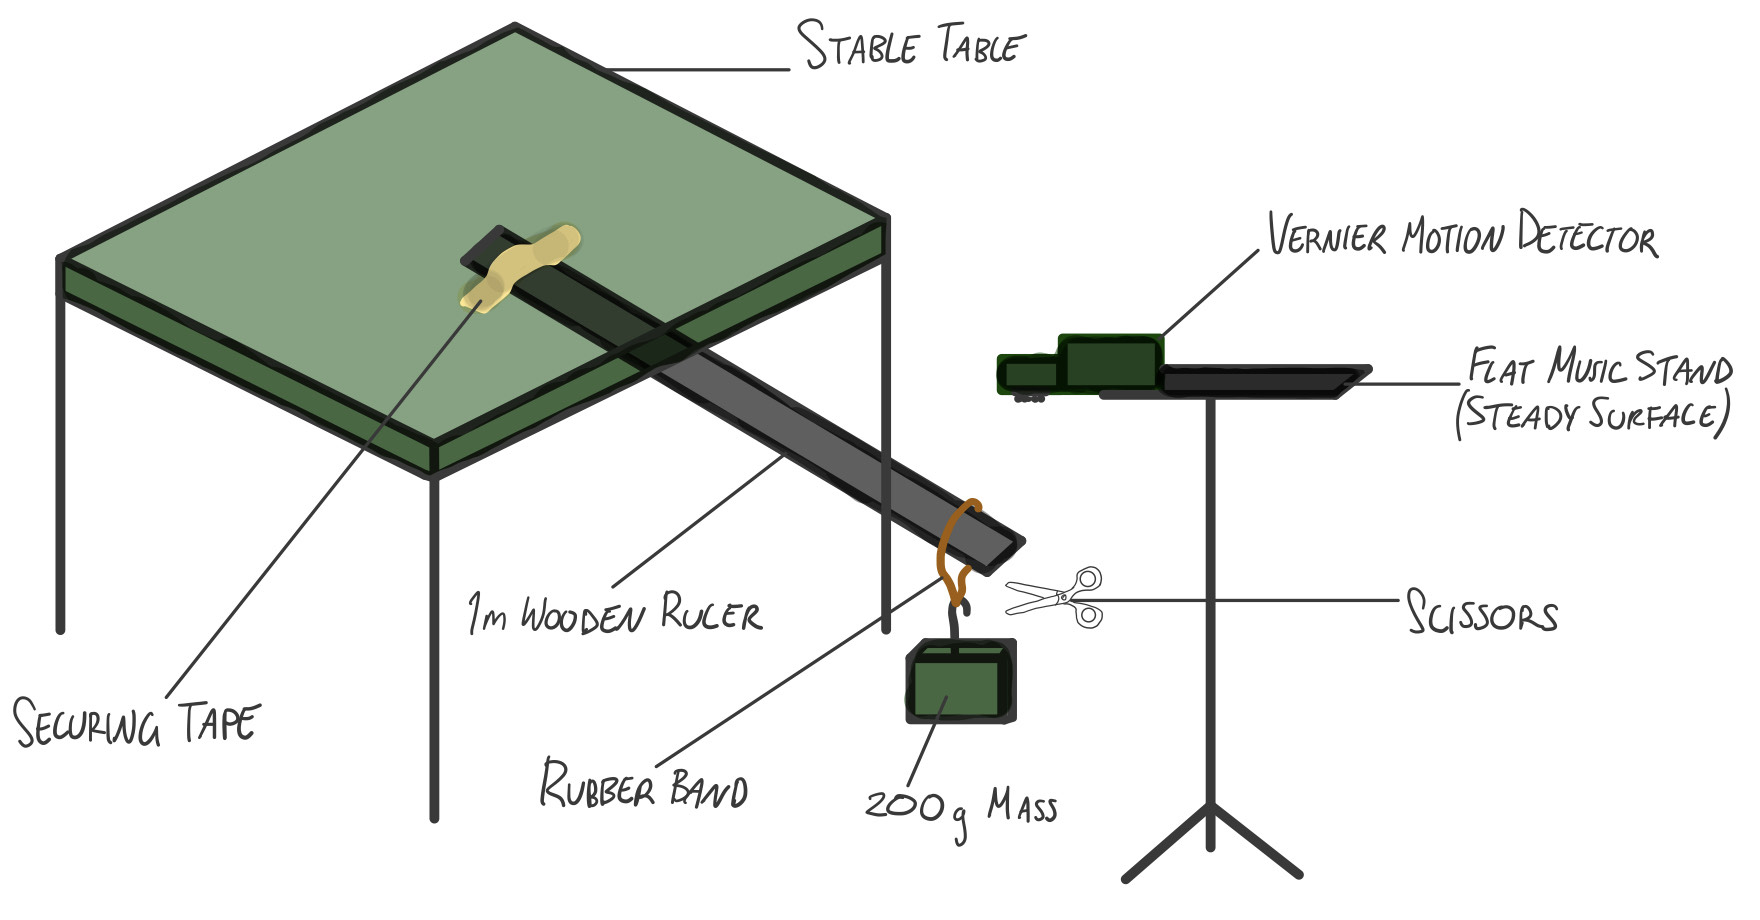
\includegraphics[width=0.65\textwidth]{images/apparatus.jpg}
    \caption{Experimental set up with model plane wing system and motion detector}
    \label{fig:apparatus}
\end{figure}


\subsection{Procedure}
\begin{enumerate}
    \item Attach the motion detector ($\pm 0.001 \frac{m}{s^2}$) to a stable and easily movable surface (such as a music stand) with the recording side facing down. 
    \item\label{initial} Secure the meter ruler ($\pm 0.05$ cm) on the edge of a stable surface, with 90.00 cm of the ruler over the air. Taping down and/or using a counterweight on the end of the ruler is recommended to maintain a stable position. 
    \item Move the motion detector directly above the edge of the ruler at reasonable height (allow about 30 cm vertical distance between the ruler and motion detector).
    \item\label{initial.trial} Hook the 200 g ($\pm0.05$ g) mass onto the rubber band, and suspend it 5.00 cm ($\pm 0.05$ cm) from the end of the ruler by placing the rubber band over the 5.00 cm mark on the ruler. If the rubber band begins to slip down, secure it with tape. 
    \item Ensure the motion detector is set to record at 100 iterations per second, and the ruler is not moving. Calibrate the motion detector to 0 and begin recording.
    \item Using scissors, cut the rubber band, allowing the weight to drop to the floor and the end of the ruler to oscillate freely. It is recommended to hold the ruler down to the table for stability.
    \item\label{final.trial} Stop recording the data once the oscillations have become insignificant (minimal vibrations).
    \item\label{final} Repeat steps \ref{initial.trial} to \ref{final.trial}, 6 more times for a total of 7 trials.
    \item Repeat steps \ref{initial} to \ref{final}, 4 more times, reducing the length of the portion of the ruler suspended in the air by 10.00 cm ($\pm 0.05$ cm) each time until 50.00 cm is reached.
\end{enumerate}

\subsection{Safety and Ethics}
There is a slight risk with the 200 g mass dropping to the floor so the floor must be cleared to ensure the mass does not break anything upon contact. Additionally, care must be taken when the mass is released as the plane wing model will begin to oscillate freely and can hit anything that is within 30 cm above or below it so these areas must be cleared as well. As the majority of the equipment in the experiment is reusable and no living organisms are involved, there are limited environmental and ethical concerns.

\section{Data Collection}

\subsection{Raw Data}

\begin{figure}[H]
     \centering
     \caption{Representative sample of the raw data as graphs generated by LoggerPro showing 2/7 trials of the model plane wing lengths (50.00 cm, 60.00 cm, 70.00 cm, 80.00 cm, 90.00 cm) and their acceleration-time graphs with qualitative observations.}
     \begin{subfigure}[b]{\textwidth}
         \centering
         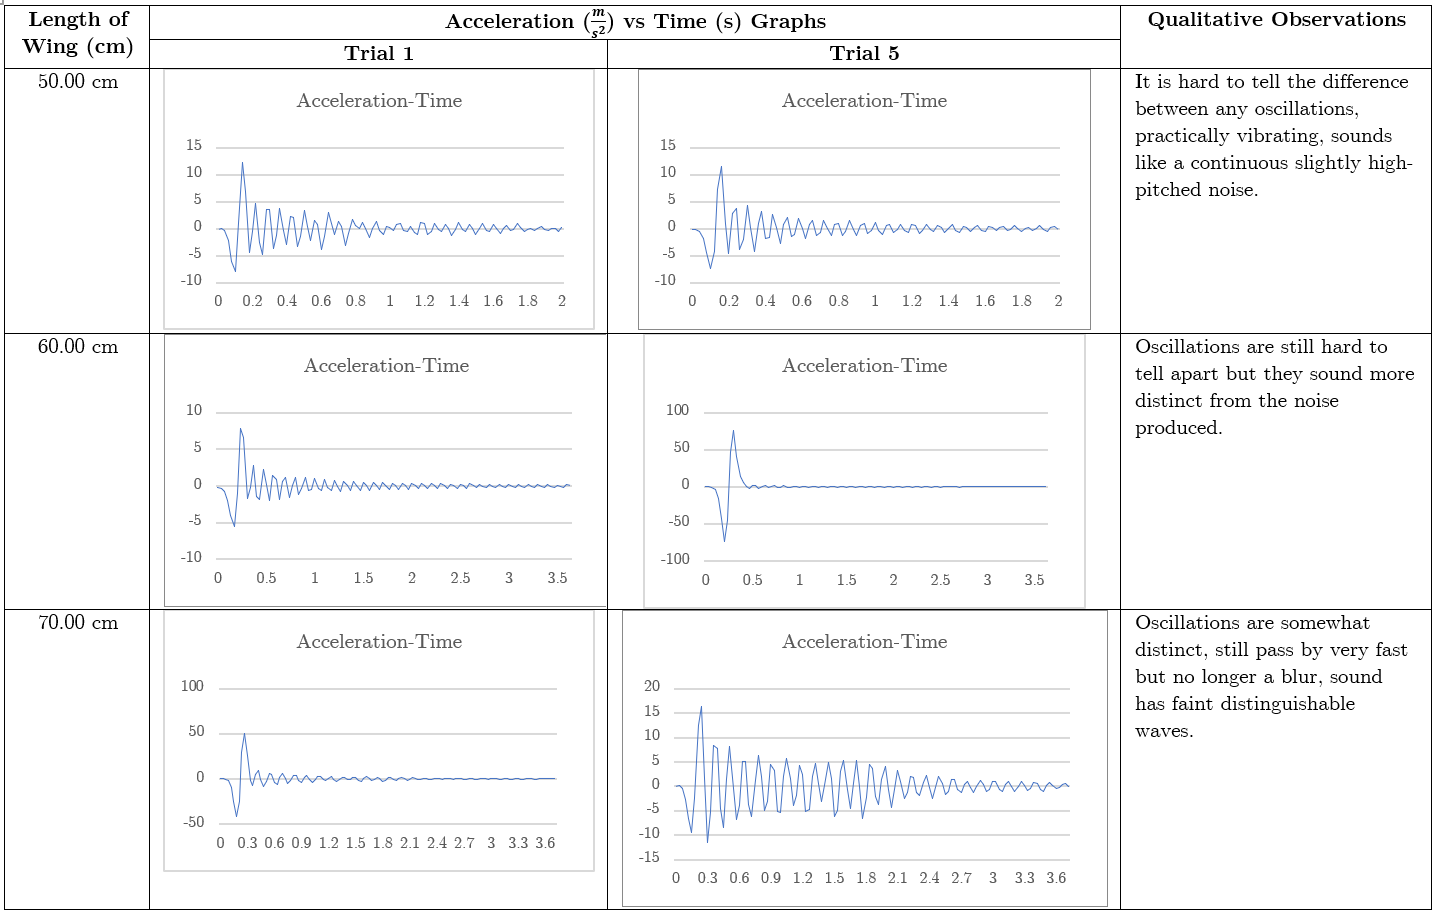
\includegraphics[width=\textwidth]{images/raw1.png}
     \end{subfigure}
     \hfill
     \begin{subfigure}[b]{\textwidth}
         \centering
         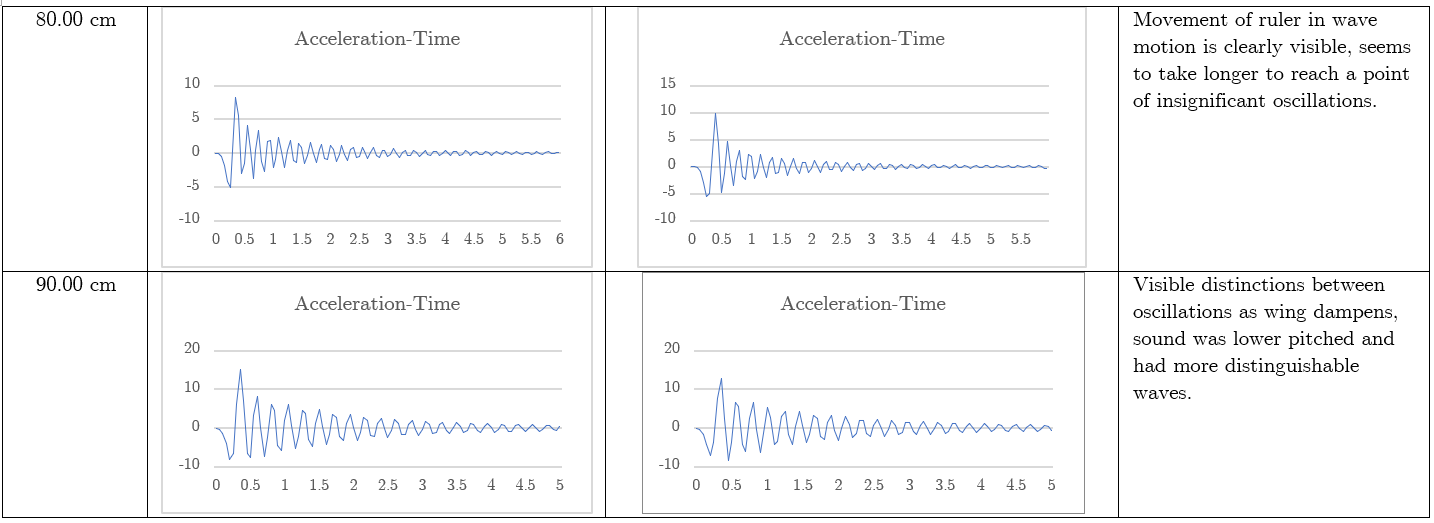
\includegraphics[width=\textwidth]{images/raw 2.png}
     \end{subfigure}
     \hfill
    \label{fig:raww}
\end{figure}


\subsection{Processed Data}

\begin{table}[H]
\centering
\caption{Processed data showing length of the model plane wing (50.00 cm, 60.00 cm, 70.00 cm, 80.00cm, 90.00 cm) and the mean values for the amplitudes of the first two peaks ($A_1$ and $A_2$), the calculated logarithmic decrement ($\delta$) and damping ratio ($\zeta$) and the standard deviation for $\zeta$.}
\begin{tabular}{|ccccccc|}
\hline
\rowcolor[HTML]{C0C0C0} 
{\color[HTML]{000000} \begin{tabular}[c]{@{}c@{}}Length \\ ($\pm 0.05$ cm)\end{tabular}} & {\color[HTML]{000000} \begin{tabular}[c]{@{}c@{}}Mean $A_1$ \\ ($\pm 0.001 \frac{m}{s^2}$)\end{tabular}} & {\color[HTML]{000000} \begin{tabular}[c]{@{}c@{}}Mean $A_2$ \\ ($\pm 0.001 \frac{m}{s^2}$)\end{tabular}} & {\color[HTML]{000000} \begin{tabular}[c]{@{}c@{}} $\delta$  \\ ($\pm 0.001$)\end{tabular}} & {\color[HTML]{000000} \begin{tabular}[c]{@{}c@{}} $\zeta$ \\ ($\pm 0.001$)\end{tabular}} & \begin{tabular}[c]{@{}c@{}} $\zeta^2$ \\ ($\pm 0.001$)\end{tabular} & STDEV \\ \hline
50.00   & 8.636                                                                                 & 3.192                                                                           & 1.061                                                                            & 0.167                                                                       & 0.028                                                 & 0.006                                                                       \\
\rowcolor[HTML]{EFEFEF} 
60.00  
& 10.947                                                                                & 3.923                                                                           & 1.024                                                                            & 0.159                                                                       & 0.025                                                 & 0.002\\
70.00                                                                         & 6.451                                                                                 & 2.836                                                                           & 0.822                                                                            & 0.129                                                                       & 0.017                                                 & 0.002 \\
\rowcolor[HTML]{EFEFEF} 
80.00 
& 14.033                                                                                & 7.230                                                                           & 0.668                                                                            & 0.101                                                                       & 0.010                                                 & 0.001 \\
90.00                                                                         & 14.182                                                                                & 7.853                                                                           & 0.583                                                                            & 0.088                                                                       & 0.008                                                 & 0.002 \\ \hline
\end{tabular}
\end{table}

The first two peak amplitudes, $A_1$ and $A_2$, for each trial were found by qualitatively finding the data points that corresponded to the first two maxima in the acceleration-time graphs produced by LoggerPro when measuring with the motion detector. For each length, the mean peak amplitudes were found by taking the sum of all trials for each respective peak and then dividing it by the total number of trials as shown below for $A_1$ of the length 90.00 cm:

\begin{equation}
    \frac{(16.254 + 11.380 + 12.319 + 14.641 + 15.747 + 15.895 + 13.039)}{7} = 14.182
\end{equation}

The logarithmic decrement, $\delta$, for each length was then found by subtracting the natural logarithm of the mean $A_2$ from the natural logarithm of the mean of $A_2$ for that length, as outlined by \citeauthor{miller_mattuck}. This process is demonstrated for the logarithmic decrement of the length 90.00 cm.

\vspace{-5mm}

\begin{equation}
    ln(14.182) - ln(7.853) = 0.583
\end{equation}

From the calculations for the logarithmic decrement, the damping ratio, $\zeta$, can be found from Equation \ref{zeta in delta}, as outlined by \citeauthor{miller_mattuck}. This ratio describes how the oscillations of the plane wing system decay. Using the logarithmic decrement for the length 90.00 cm, we can find its damping ratio as shown below:

\vspace{-10mm}

\begin{equation}
    \zeta = \frac{0.583}{\sqrt{4\pi^2+0.583^2}} = 0.088
\end{equation}

According to the theoretically derived relationship between the spring constant and damping ratio, the spring constant varies directly with the square of the damping ratio, hence $\zeta$ was then squared to produce a linear relationship when graphed as shown below:

\vspace{-5mm}

\begin{equation}
    \zeta^2 = 0.08815^2 = 0.00777
\end{equation}

Finally, the standard deviation was found by taking the mean between the standard deviation of $A_1$ across all seven trials within each length, and that of $A_2$ found by applying the =STDEV function in Excel as shown:

\vspace{-10mm}

$$
\begin{array}{l}
    \text{STDEV}(8.288,9.906,8.208,8.567,7.604,8.757,9.118) \\
    + \text{ STDEV}(4.030,4.590,1.856,2.729,3.921,1.549,3.666) \\
    \div \text{ 2 } = 0.002
 \end{array} 
$$

\subsection{Graph}

\begin{figure}[H]
    \centering
    \caption{The relationship between the model plane wing length (cm) and the square of the calculated damping ratio ($\zeta$), with error bars showing standard deviation.}
    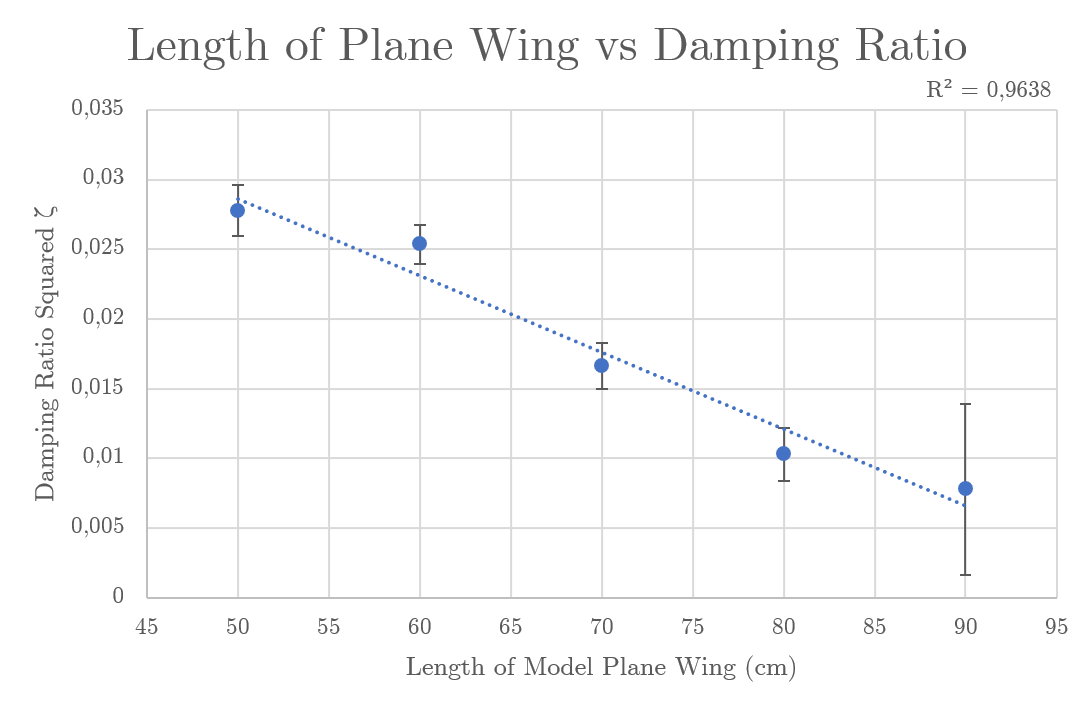
\includegraphics[width=0.65\textwidth]{images/graph.png}
    \label{fig:processed graph}
\end{figure}

\vspace{-10mm}

\section{Analysis}

The relationship between an increasing length of the model plane wing and the square of the respective damping ratio shows a strong negative linear relationship as seen in Figure \ref{fig:processed graph}. As the length of the plane wing model increases from 50.00 cm to 90.00 cm, the square of the damping ratio significantly decreases from 0.028 to 0.008, illustrating this inverse relationship. 

The high coefficient of determination value, $R^2 = 0.9638$ (Figure \ref{fig:processed graph}), demonstrates a strong relationship between the data and the plotted linear regression. This indicates that the variance in the data is accurately predicted by the linear trend, hence it is a strong statistical model. However, it is important to note how for some data points, there is an overlap of error bars. This indicates that some of the data may not be statistically significant. For example, the lower range of the calculated damping ratio for the 50.00 cm plane wing coincides with that of the upper range of the 60.00 cm plane wing showing how the damping ratios for these lengths are not exclusive. It is even more important to note the significant standard deviation, as represented by the error bars for the 90.00 cm plane wing length. This can be understood in the context that because the spring constant was relatively the lowest for this length, small changes in the amount of force applied would have a larger impact on the displacement, and hence, would be more likely to produce a larger range of data points. Nonetheless, there is an evident inverse relationship between an increasing plane wing length and the square of the damping ratio. 

The qualitative data recorded supports this negative linear trend as seen in Figure \ref{fig:raww}. At smaller plane wing lengths, the oscillations are noted as vibrations that rapidly diminish. This supports the data indicating a higher damping ratio, as these oscillations are damped faster and thus the plane wing returns to equilibrium quicker. Similarly, for longer plane wing lengths, the observations note that not only are the oscillations distinct, but they visibly take longer to reduce in intensity, which supports the data that shows a smaller damping ratio, indicating the wing would have to undergo more oscillations until it is damped. 

\vspace{-5mm}

\section{Evaluation and Conclusion}

\subsection{Conclusion}
This experiment investigated how an increasing plane wing length, as modelled by a wooden ruler, affects the damping ratio of the underdamped system of a plane wing. The experimental data supports the hypothesis which predicted an inverse relationship between the length of the plane wing and the damping ratio. By measuring the acceleration of the model wing when displaced by the same force at different lengths, the damping ratio was determined from the change in maxima of the oscillations. From this, a negative linear relationship was concluded between the variables which was supported by the qualitative observations and was determined to show statistical significance through a high coefficient of determination. 

These conclusions align with the theoretical basis that, for a simplified system, an increase in plane wing length will decrease the spring constant, and hence decrease the natural frequency of the system, as shown in Equation \ref{wnk} (\citeauthor{hallauer_2022}). As proved by \citeauthor{miller_mattuck}, a decrease in the natural frequency of an underdamped system will cause the damping ratio decrease accordingly because the damping ratio needed to maintain the relative damped frequency will decrease. Hence, corroborating the link found between an increase in length of a plane wing and the decrease in damping ratio demonstrated in this investigation.

\vspace{-5mm}

\subsection{Strengths and Limitations}

Certain aspects of the design of this experiment provided a strong basis for the investigation. The method of displacing the plane wing model by suspending a mass from a rubber band that was cut proved extremely effective. By cutting the rubber band that held the mass, the net downwards force was removed instantaneously, allowing it to not interfere with the oscillations of the plane wing. Furthermore, it allowed a constant force to be applied across all trials and lengths, which meant the effect of the length of the plane wing could be isolated against the spring constant. Simultaneously, the use of a motion detector to measure the oscillations was a very effective way of determining the damping ratio because of its accuracy. Even when the oscillations were not visibly distinguishable, the motion detector was still able to accurately capture the movement. This resulted in generally a low standard deviation across the lengths, demonstrating the reliability of the results obtained. 

However, the simplification of the experiment also posed great limitations. By using a 1 m wooden ruler as a model plane wing, only a very small range of data could be collected. At lengths shorter than 50.00 cm for the model plane wing, the oscillations were too small for the motion detector to register. As a result, the complete range of the damping ratio for an underdamped system, between 0 and 1, was not represented. Therefore, the conclusions from this experiment, while theoretically supported, cannot necessarily be extrapolated for a system approaching critical damping of 1. Furthermore, this experiment relied on the qualitative determination of the maximas, $A_1$ and $A_2$, for the logarithmic decrement. This posed potential inaccuracies in determining the true maxima, and can be indicative of the large standard deviation seen for the length of 90.00 cm. 

\vspace{-5mm}

\subsection{Extensions}
This experiment used a highly simplified model of a plane wing, where manipulating the length would only have an effect on the natural frequency. However, changing the length of a plane wing on an aircraft also impacts the structural damping and aerodynamic effects of the wing. Hence, extensions for the experiment include testing length variations of more accurately modelled plane wings, in which their structural damping is affected, as well as plane wings within a wind tunnel, where the added effects of a dynamic fluid further interfere with the damping ratio, in a more realistic manner as exhibited by plane wings while in flight. 


\pagebreak
\printbibliography

\end{document}